\RequirePackage[l2tabu, orthodox]{nag}

%\documentclass[]{article}
\documentclass[11pt]{scrartcl}
\usepackage[usename, dvipsnames]{xcolor}
\usepackage[pdfencoding=auto]{hyperref}
\usepackage[msc-links]{amsrefs}
\usepackage{cleveref} % use \cref{}, automatically deduces theorem, proposition, etc
\usepackage[mathletters]{ucs}
\usepackage[utf8]{inputenc}
\usepackage[T1]{fontenc}
\usepackage{datetime}

\usepackage{array}
\usepackage{mathtools}
\usepackage{amsmath, amsthm, amssymb, amsfonts, amsxtra, amscd, thmtools}
\let\proof\relax
\let\endproof\relax

% Boxes around theorem environments.
\usepackage[many]{tcolorbox}

\usepackage{color}
%\usepackage{unicode-math}
\usepackage{newunicodechar}
\newunicodechar{ε}{\varepsilon}
\newunicodechar{δ}{\delta}
\newunicodechar{µ}{\mu}
\newunicodechar{→}{\to}
\newunicodechar{≤}{\leq}
\newunicodechar{∈}{\in}
\newunicodechar{⊆}{\subseteq}
\newunicodechar{Λ}{\Lambda}
\newunicodechar{∞}{\infty}
\newunicodechar{×}{\times}
\everymath{\displaystyle}



\usepackage{microtype}
\usepackage[pdfencoding=auto]{hyperref}
\usepackage{bookmark}
\usepackage{booktabs}
\usepackage{todonotes}
\usepackage[msc-links]{amsrefs}
\usepackage{cleveref} % use \cref{}, automatically deduces theorem, proposition, etc
\usepackage{csquotes}
\usepackage{longtable}
\usepackage{tabularx}
\usepackage{bbm}
% Creating multiple types of index
\usepackage{imakeidx}

% Remove indentation for new paragraphs
\usepackage{parskip}
% But leave space before amsthm environments
\makeatletter
\def\thm@space@setup{%
  \thm@preskip=2em
  \thm@postskip=2em
}
\makeatother


\usepackage{stmaryrd}
\usepackage{adjustbox}
\usepackage{centernot}
% \centernot\whatever


% Better indicator function
\usepackage{bbm}
\newcommand{\indic}[1]{\mathbbm{1} \left[ {#1} \right] }

% Highlight quote
\usepackage{environ}
\definecolor{camel}{rgb}{0.76, 0.6, 0.42}
\definecolor{babyblue}{rgb}{0.54, 0.81, 0.94}
\definecolor{block-gray}{gray}{0.85}
\NewEnviron{myblock}
{\colorbox{block-gray}{%
\parbox{\dimexpr\linewidth-2\fboxsep\relax}{%
\small\addtolength{\leftskip}{10mm}
\addtolength{\rightskip}{10mm}
\BODY}}
}
\renewcommand{\quote}{\myblock}
\renewcommand{\endquote}{\endmyblock}

% Nice math font that journals use
%\usepackage[lite]{mtpro2}
%\usepackage{mathrsfs}
%\usepackage{mathptmx}
\usepackage{lmodern}
%\usepackage[sc]{mathpazo}

% Theorem Styles
\usepackage[framemethod=tikz]{mdframed}

\theoremstyle{definition}
\newtheorem{exercise}{Exercise}[section]
\newtheorem{solution}{Solution}

% Theorem Style
\newtheoremstyle{theorem}% name
  {0em}%         Space above, empty = `usual value'
  {1em}%         Space below
  {\normalfont}% Body font
  {\parindent}%         Indent amount (empty = no indent, \parindent = para indent)
  {\bfseries}% Thm head font
  {.}%        Punctuation after thm head
  {\newline}% Space after thm head: \newline = linebreak
  {\thmname{#1}\thmnumber{ #2}\thmnote{\itshape{(#3)}}}%
\theoremstyle{theorem}
\tcolorboxenvironment{theorem}{
  boxrule=0pt,
  boxsep=0pt,
  breakable,
  enhanced jigsaw,
  fonttitle={\large\bfseries},
  opacityback=0.8,
  colframe=cyan,
  borderline west={4pt}{0pt}{orange},
  attach title to upper={}
}
\newtheorem{theorem}{Theorem}[section]

% Proposition Style
\tcolorboxenvironment{proposition}{
  boxrule=1pt,
  boxsep=0pt,
  breakable,
  enhanced jigsaw,
  opacityback=0.0,
  colframe=cyan
}
\newtheorem{proposition}[theorem]{Proposition}
\tcolorboxenvironment{lemma}{
  boxrule=1pt,
  boxsep=0pt,
  breakable,
  enhanced jigsaw,
  opacityback=0.2,
  colframe=cyan
}
\newtheorem{lemma}[theorem]{Lemma}
% Claim
\tcolorboxenvironment{claim}{
  boxrule=1pt,
  boxsep=0pt,
  breakable,
  enhanced jigsaw,
  opacityback=0.2,
  colframe=cyan
}
\newtheorem{claim}[theorem]{Claim}


% Corollary
\tcolorboxenvironment{corollary}{
  colback=cyan,
  boxrule=1pt,
  boxsep=0pt,
  breakable,
  enhanced jigsaw,
  opacityback=0.1,
  colframe=cyan
}
\newtheorem{corollary}[theorem]{Corollary}

% Proof Style
\newtheoremstyle{proof}% name
  {0em}%         Space above, empty = `usual value'
  {2em}%         Space below
  {\normalfont}% Body font
  {\parindent}%         Indent amount (empty = no indent, \parindent = para indent)
  {\itshape}% Thm head font
  {.}%        Punctuation after thm head
  {\newline}% Space after thm head: \newline = linebreak
  {\thmname{#1} \thmnote{\itshape{(#3)}}}%         Thm head spec
\theoremstyle{proof}
\tcolorboxenvironment{proof}{
  colback=camel,
  opacityfill=0.25,
  boxrule=1pt,
  boxsep=0pt,
  breakable,
  enhanced jigsaw
}
\newtheorem*{pf}{Proof}
\newenvironment{proof}
{\pushQED{$\qed$}\pf}
{\par\popQED\endpf}

% Definition Style
\newtheoremstyle{definition}% name
  {0em}%         Space above, empty = `usual value'
  {2em}%         Space below
  {\normalfont}% Body font
  {\parindent}%         Indent amount (empty = no indent, \parindent = para indent)
  {\bfseries}% Thm head font
  {.}%        Punctuation after thm head
  {\newline}% Space after thm head: \newline = linebreak
  {}%         Thm head spec
\theoremstyle{definition}
\tcolorboxenvironment{definition}{
  colback=babyblue,
  boxrule=0pt,
  boxsep=0pt,
  opacityfill=0.45,
  breakable,
  enhanced jigsaw,
  borderline west={4pt}{0pt}{blue},
  colbacktitle={babyblue},
  coltitle={black},
  fonttitle={\large\bfseries},
  attach title to upper={},
}
\newtheorem{definition}{Definition}[theorem]

% Break Environment
\makeatletter
\newtheoremstyle{break}% name
  {}%         Space above, empty = `usual value'
  {2em}%         Space below
  {
    \addtolength{\@totalleftmargin}{2.5em}
    \addtolength{\linewidth}{-2.5em}
    \parshape 1 2.5em \linewidth
  }% Body font
  {}%         Indent amount (empty = no indent, \parindent = para indent)
  {\bfseries}% Thm head font
  {.}%        Punctuation after thm head
  {\newline}% Space after thm head: \newline = linebreak
  {}%         Thm head spec
\makeatother

\theoremstyle{break}
\newtheorem{example}{Example}[section]

% Problem Style
\newtheoremstyle{problem} % name
  {0em}                   % Space above, empty = `usual value'
  {2em}                   % Space below
  {\normalfont}           % Body font
  {\parindent}            % Indent amount (empty = no indent, \parindent = para indent)
  {\itshape}              % Thm head font
  {}                      % Punctuation after thm head
  {\newline}              % Space after thm head: \newline = linebreak
  {\thmnote{\itshape{(#3)}}}     % Thm head spec
\theoremstyle{problem}
\tcolorboxenvironment{problem}{
  boxrule=1pt,
  boxsep=0pt,
  breakable,
  enhanced jigsaw,
  opacityback=0.0,
  colframe=cyan
}
\newtheorem{problem}{Problem}


%Pagination stuff.
\setlength{\topmargin}{-.3 in}
\setlength{\oddsidemargin}{0in}
\setlength{\evensidemargin}{0in}
\setlength{\textheight}{9.in}
\setlength{\textwidth}{6.5in}
% \pagestyle{empty} %removes page numbers.

% Inkscape figures from Vim
\usepackage{import}
\usepackage{pdfpages}
\usepackage{transparent}

\newcommand{\incfig}[1]{%
    \def\svgwidth{\columnwidth}
    \import{./figures/}{#1.pdf_tex}
}
%\pdfsuppresswarningpagegroup=1

% Pandoc-specific fixes
\providecommand{\tightlist}{%
  \setlength{\itemsep}{0pt}\setlength{\parskip}{0pt}}

% Tikz and Graphics
\usepackage{amscd}
\usepackage{tikz}
\usetikzlibrary{arrows, arrows.meta, cd, fadings, patterns, calc, decorations.markings, matrix, positioning}
\tikzfading[name=fade out, inner color=transparent!0, outer color=transparent!100]
\usepackage{pgfplots}
\pgfplotsset{compat=1.16}
\usepackage[inline]{asymptote}
\usepackage{tikz-layers}

%\usepackage{nath}
%\delimgrowth=1
\DeclarePairedDelimiter\qty{(}{)}

% Major Macros
\usepackage{graphicx}
\usepackage{float}
\DeclareFontFamily{U}{mathx}{\hyphenchar\font45}
\DeclareFontShape{U}{mathx}{m}{n}{
      <5> <6> <7> <8> <9> <10>
      <10.95> <12> <14.4> <17.28> <20.74> <24.88>
      mathx10
      }{}
\DeclareSymbolFont{mathx}{U}{mathx}{m}{n}
\DeclareMathSymbol{\bigtimes}{1}{mathx}{"91}

% Wide tikz equations
\newsavebox{\wideeqbox}
\newenvironment{wideeq}
  {\begin{displaymath}\begin{lrbox}{\wideeqbox}$\displaystyle}
  {$\end{lrbox}\makebox[0pt]{\usebox{\wideeqbox}}\end{displaymath}}



% Fancy chapter headers and footers
\usepackage{fancyhdr}

\pagestyle{fancy}
\fancyhf{}
\fancyhead[LE,RO]{\title}
\fancyhead[RE,LO]{\rightmark}
\fancyfoot[CE,CO]{\leftmark}
\fancyfoot[LE,RO]{\thepage}

\renewcommand{\headrulewidth}{2pt}
\renewcommand{\footrulewidth}{1pt}

% List of Theorems Attempt
\usepackage{etoolbox}
\makeatletter
\patchcmd\thmtlo@chaptervspacehack
  {\addtocontents{loe}{\protect\addvspace{10\p@}}}
  {\addtocontents{loe}{\protect\thmlopatch@endchapter\protect\thmlopatch@chapter{\thechapter}}}
  {}{}
\AtEndDocument{\addtocontents{loe}{\protect\thmlopatch@endchapter}}
\long\def\thmlopatch@chapter#1#2\thmlopatch@endchapter{%
  \setbox\z@=\vbox{#2}%
  \ifdim\ht\z@>\z@
    \hbox{\bfseries\chaptername\ #1}\nobreak
    #2
    \addvspace{10\p@}
  \fi
}
\def\thmlopatch@endchapter{}

\makeatother
\renewcommand{\thmtformatoptarg}[1]{ -- #1}
%\renewcommand{\listtheoremname}{List of definitions}

\newcommand{\ext}{\operatorname{Ext}}
\newcommand{\Ext}{\operatorname{Ext}}
\def\Endo{\operatorname{End}}
\def\Ind{\operatorname{Ind}}
\def\ind{\operatorname{Ind}}
\def\coind{\operatorname{Coind}}
\def\Res{\operatorname{Res}}
\def\Hol{\operatorname{Hol}}
\def\res{\operatorname{Res}}
\def\endo{\operatorname{End}}
\def\ind{\operatorname{Ind}}
\renewcommand{\AA}[0]{{\mathbb{A}}}
\DeclareMathOperator{\Exists}{\exists}
\DeclareMathOperator{\Forall}{\forall}
\newcommand{\Af}[0]{{\mathbb{A}}}
\newcommand{\CC}[0]{{\mathbb{C}}}
\newcommand{\CP}[0]{{\mathbb{CP}}}
\newcommand{\DD}[0]{{\mathbb{D}}}
\newcommand{\FF}[0]{{\mathbb{F}}}
\newcommand{\GF}[0]{{\mathbb{GF}}}
\newcommand{\GG}[0]{{\mathbb{G}}}
\newcommand{\HH}[0]{{\mathbb{H}}}
\newcommand{\HP}[0]{{\mathbb{HP}}}
\newcommand{\KK}[0]{{\mathbb{K}}}
\newcommand{\kk}[0]{{\Bbbk}}
\newcommand{\bbm}[0]{{\mathbb{M}}}
\newcommand{\NN}[0]{{\mathbb{N}}}
\newcommand{\OP}[0]{{\mathbb{OP}}}
\newcommand{\PP}[0]{{\mathbb{P}}}
\newcommand{\QQ}[0]{{\mathbb{Q}}}
\newcommand{\RP}[0]{{\mathbb{RP}}}
\newcommand{\RR}[0]{{\mathbb{R}}}
\newcommand{\SpSp}[0]{{\mathbb{S}}}
\renewcommand{\SS}[0]{{\mathbb{S}}}
\newcommand{\TT}[0]{{\mathbb{T}}}
\newcommand{\ZZ}[0]{{\mathbb{Z}}}
\newcommand{\ZnZ}[0]{\mathbb{Z}/n\mathbb{Z}}
\newcommand{\ZpZ}[0]{\mathbb{Z}/p\mathbb{Z}}
\newcommand{\Qp}[0]{\mathbb{Q}_{(p)}}
\newcommand{\Zp}[0]{\mathbb{Z}_{(p)}}
\newcommand{\Arg}[0]{\mathrm{Arg}}
\newcommand{\PGL}[0]{\mathrm{PGL}}
\newcommand{\GL}[0]{\mathrm{GL}}
\newcommand{\Gl}[0]{\mathrm{GL}}
\newcommand{\gl}[0]{\mathrm{GL}}
\newcommand{\mat}[0]{\mathrm{Mat}}
\newcommand{\Mat}[0]{\mathrm{Mat}}
\newcommand{\Rat}[0]{\mathrm{Rat}}
\newcommand{\Perv}[0]{\mathrm{Perv}}
\newcommand{\Gal}[0]{\mathrm{Gal}}
\newcommand{\Hilb}[0]{\mathrm{Hilb}}
\newcommand{\Quot}[0]{\mathrm{Quot}}
\newcommand{\Art}[0]{\mathrm{Art}}
\newcommand{\red}[0]{\mathrm{red}}
\newcommand{\alg}[0]{\mathrm{alg}}
\newcommand{\Pic}[0]{{\mathrm{Pic}~}}
\newcommand{\lcm}[0]{\mathrm{lcm}}
\newcommand{\maps}[0]{\mathrm{Maps}}
\newcommand{\maxspec}[0]{{\mathrm{maxSpec}~}}
\newcommand{\Tr}[0]{\mathrm{Tr}}
\newcommand{\adj}[0]{\mathrm{adj}}
\newcommand{\ad}[0]{\mathrm{ad}~}
\newcommand{\ann}[0]{\mathrm{Ann}}
\newcommand{\Ann}[0]{\mathrm{Ann}}
\newcommand{\arcsec}[0]{\mathrm{arcsec}}
\newcommand{\ch}[0]{\mathrm{char}~}
\newcommand{\Sp}[0]{{\mathrm{Sp}}}
\newcommand{\syl}[0]{{\mathrm{Syl}}}
\newcommand{\txand}[0]{{\text{ and }}}
\newcommand{\codim}[0]{\mathrm{codim}}
\newcommand{\txor}[0]{{\text{ or }}}
\newcommand{\txt}[1]{{\text{ {#1} }}}
\newcommand{\Gr}[0]{{\text{Gr}}}
\newcommand{\Aut}[0]{{\mathrm{Aut}}}
\newcommand{\aut}[0]{\mathrm{Aut}}
\newcommand{\Inn}[0]{{\mathrm{Inn}}}
\newcommand{\Out}[0]{{\mathrm{Out}}}
\newcommand{\mltext}[1]{\left\{\begin{array}{c}#1\end{array}\right\}}
\newcommand{\Fun}[0]{{\text{Fun}}}
\newcommand{\SL}[0]{{\text{SL}}}
\newcommand{\PSL}[0]{{\text{PSL}}}
\newcommand{\SO}[0]{{\text{SO}}}
\newcommand{\SU}[0]{{\text{SU}}}
\newcommand{\SP}[0]{{\text{SP}}}
\newcommand{\per}[0]{{\text{Per}}}
\newcommand{\loc}[0]{{\text{loc}}}
\newcommand{\Top}[0]{{\text{Top}}}
\newcommand{\Sch}[0]{{\text{Sch}}}
\newcommand{\sch}[0]{{\text{Sch}}}
\newcommand{\Set}[0]{{\text{Set}}}
\newcommand{\Sets}[0]{{\text{Set}}}
\newcommand{\Grp}[0]{{\text{Grp}}}
\newcommand{\Groups}[0]{{\text{Groups}}}
\newcommand{\Homeo}[0]{{\text{Homeo}}}
\newcommand{\Diffeo}[0]{{\text{Diffeo}}}
\newcommand{\MCG}[0]{{\text{MCG}}}
\newcommand{\set}[0]{{\text{Set}}}
\newcommand{\Tor}[0]{\text{Tor}}
\newcommand{\sets}[0]{{\text{Set}}}
\newcommand{\Sm}[0]{{\text{Sm}_k}}
\newcommand{\orr}[0]{{\text{ or }}}
\newcommand{\annd}[0]{{\text{ and }}}
\newcommand{\bung}[0]{\text{Bun}_G}
\newcommand{\const}[0]{{\text{const.}}}
\newcommand{\disc}[0]{{\text{disc}}}
\newcommand{\op}[0]{^\text{op}}
\newcommand{\id}[0]{\text{id}}
\newcommand{\im}[1]{\mathrm{im}({#1})}
\newcommand{\pt}[0]{{\{\text{pt}\}}}
\newcommand{\sep}[0]{^\text{sep}}
% \newcommand{\st}[0]{~{\text{s.t.}}~}
\newcommand{\tors}[0]{{\text{tors}}}
\newcommand{\tor}[0]{\text{Tor}}
\newcommand{\height}[0]{\text{ht}}
\newcommand{\cpt}[0]{\text{compact}}
\newcommand{\abs}[1]{{\left\lvert {#1} \right\rvert}}
\newcommand{\stack}[1]{\mathclap{\substack{ #1 }}} 
\newcommand{\qtext}[1]{{\quad \text{#1} \quad}}
\newcommand{\qst}[0]{{\quad \text{such that} \quad}}
\newcommand{\actsonl}[0]{\curvearrowleft}
\newcommand{\actson}[0]{\curvearrowright}
\newcommand{\bd}[0]{{\del}}
\newcommand{\bigast}[0]{{\mathop{\Large \ast}}}
\newcommand{\coker}[0]{\operatorname{coker}}
\newcommand{\cok}[0]{\operatorname{coker}}
\newcommand{\conjugate}[1]{{\overline{{#1}}}}
\newcommand{\converges}[1]{\overset{#1}}
\newcommand{\correspond}[1]{\theset{\substack{#1}}}
\newcommand{\cross}[0]{\times}
\newcommand{\by}[0]{\times}
\newcommand{\dash}[0]{{\hbox{-}}}
\newcommand{\dd}[2]{{\frac{\partial #1}{\partial #2}\,}}
\newcommand{\definedas}[0]{\coloneqq}
\newcommand{\da}[0]{\coloneqq}
\newcommand{\del}[0]{{\partial}}
\newcommand{\directlim}[0]{\varinjlim}
\newcommand{\disjoint}[0]{{\coprod}}
\newcommand{\divides}[0]{{~\Bigm|~}}
\newcommand{\dual}[0]{^\vee}
\newcommand{\sm}[0]{\setminus}
\newcommand{\smz}[0]{\setminus\theset{0}}
\newcommand{\eps}[0]{\varepsilon}
\newcommand{\equalsbecause}[1] {\stackrel{\mathclap{\scriptscriptstyle{#1}}}{=}}
\newcommand{\floor}[1]{{\left\lfloor #1 \right\rfloor}}
\DeclarePairedDelimiter{\ceil}{\lceil}{\rceil}
\newcommand{\from}[0]{\leftarrow}
\newcommand{\tofrom}[0]{\leftrightarrows}
\newcommand{\up}[0]{\uparrow}
\newcommand{\generators}[1]{\left\langle{#1}\right\rangle}
\newcommand{\gs}[1]{\left\langle{#1}\right\rangle}
\newcommand{\homotopic}[0]{\simeq}
\newcommand{\injectivelim}[0]{\varinjlim}
\newcommand{\injects}[0]{\hookrightarrow}
\newcommand{\inner}[2]{{\left\langle {#1},~{#2} \right\rangle}}
\newcommand{\union}[0]{\cup}
\newcommand{\Union}[0]{\bigcup}
\newcommand{\intersect}[0]{\cap}
\newcommand{\Intersect}[0]{\bigcap}
\newcommand{\into}[0]{\to}
\newcommand{\inverselim}[0]{\varprojlim}
\newcommand{\inv}[0]{^{-1}}
\newcommand{\mfa}[0]{{\mathfrak{a}}}
\newcommand{\mfb}[0]{{\mathfrak{b}}}
\newcommand{\mfc}[0]{{\mathfrak{c}}}
\newcommand{\mff}[0]{{\mathfrak{f}}}
\newcommand{\mfi}[0]{{\mathfrak{I}}}
\newcommand{\mfm}[0]{{\mathfrak{m}}}
\newcommand{\mfn}[0]{{\mathfrak{n}}}
\newcommand{\mfp}[0]{{\mathfrak{p}}}
\newcommand{\mfq}[0]{{\mathfrak{q}}}
\newcommand{\mfr}[0]{{\mathfrak{r}}}
\newcommand{\lieb}[0]{{\mathfrak{b}}}
\newcommand{\liegl}[0]{{\mathfrak{gl}}}
\newcommand{\lieg}[0]{{\mathfrak{g}}}
\newcommand{\lieh}[0]{{\mathfrak{h}}}
\newcommand{\lien}[0]{{\mathfrak{n}}}
\newcommand{\liesl}[0]{{\mathfrak{sl}}}
\newcommand{\lieso}[0]{{\mathfrak{so}}}
\newcommand{\liesp}[0]{{\mathfrak{sp}}}
\newcommand{\lieu}[0]{{\mathfrak{u}}}
\newcommand{\nilrad}[0]{{\mathfrak{N}}}
\newcommand{\jacobsonrad}[0]{{\mathfrak{J}}}
\newcommand{\mm}[0]{{\mathfrak{m}}}
\newcommand{\pr}[0]{{\mathfrak{p}}}
\newcommand{\mapsvia}[1]{\xrightarrow{#1}}
\newcommand{\kx}[1]{k[x_1, \cdots, x_{#1}]}
\newcommand{\MM}[0]{{\mathcal{M}}}
\newcommand{\OO}[0]{{\mathcal{O}}}
\newcommand{\imaginarypart}[1]{{\mathcal{Im}({#1})}}
\newcommand{\mca}[0]{{\mathcal{A}}}
\newcommand{\mcb}[0]{{\mathcal{B}}}
\newcommand{\mcc}[0]{{\mathcal{C}}}
\newcommand{\mcd}[0]{{\mathcal{D}}}
\newcommand{\mce}[0]{{\mathcal{E}}}
\newcommand{\mcf}[0]{{\mathcal{F}}}
\newcommand{\mcg}[0]{{\mathcal{G}}}
\newcommand{\mch}[0]{{\mathcal{H}}}
\newcommand{\mci}[0]{{\mathcal{I}}}
\newcommand{\mcj}[0]{{\mathcal{J}}}
\newcommand{\mck}[0]{{\mathcal{K}}}
\newcommand{\mcl}[0]{{\mathcal{L}}}
\newcommand{\mcm}[0]{{\mathcal{M}}}
\newcommand{\mcp}[0]{{\mathcal{P}}}
\newcommand{\mcs}[0]{{\mathcal{S}}}
\newcommand{\mct}[0]{{\mathcal{T}}}
\newcommand{\mcu}[0]{{\mathcal{U}}}
\newcommand{\mcv}[0]{{\mathcal{V}}}
\newcommand{\mcx}[0]{{\mathcal{X}}}
\newcommand{\mcz}[0]{{\mathcal{Z}}}
\newcommand{\cl}[0]{\mathrm{cl}}
\newcommand{\trdeg}[0]{\mathrm{trdeg}}
\newcommand{\dist}[0]{\mathrm{dist}}
\newcommand{\Dist}[0]{\mathrm{Dist}}
\newcommand{\crit}[0]{\mathrm{crit}}
\newcommand{\diam}[0]{{\mathrm{diam}}}
\newcommand{\gal}[0]{\mathrm{Gal}}
\newcommand{\diff}[0]{\mathrm{Diff}}
\newcommand{\diag}[0]{\mathrm{diag}}
\newcommand{\soc}[0]{\mathrm{Soc}\,}
\newcommand{\hd}[0]{\mathrm{Head}\,}
\newcommand{\grad}[0]{\mathrm{grad}~}
\newcommand{\hilb}[0]{\mathrm{Hilb}}
\newcommand{\minpoly}[0]{{\mathrm{minpoly}}}
\newcommand{\Hom}[0]{{\mathrm{Hom}}}
\newcommand{\Map}[0]{{\mathrm{Map}}}
\newcommand{\multinomial}[1]{\left(\!\!{#1}\!\!\right)}
\newcommand{\nil}[0]{{\mathrm{nil}}}
\newcommand{\normalneq}{\mathrel{\reflectbox{$\trianglerightneq$}}}
\newcommand{\normal}[0]{{~\trianglelefteq~}}
\newcommand{\norm}[1]{{\left\lVert {#1} \right\rVert}}
\newcommand{\pnorm}[2]{{\left\lVert {#1} \right\rVert}_{#2}}
\newcommand{\notdivides}[0]{\nmid}
\newcommand{\onto}[0]{\twoheadhthtarrow}
\newcommand{\ord}[0]{{\mathrm{Ord}}}
\newcommand{\pic}[0]{{\mathrm{Pic}~}}
\newcommand{\projectivelim}[0]{\varprojlim}
\newcommand{\rad}[0]{{\mathrm{rad}~}}
\newcommand{\ralg}[0]{\mathrm{R-alg}}
\newcommand{\kalg}[0]{k\dash\mathrm{alg}}
\newcommand{\rank}[0]{\operatorname{rank}}
\newcommand{\realpart}[1]{{\mathcal{Re}({#1})}}
\newcommand{\Log}[0]{\mathrm{Log}}
\newcommand{\reg}[0]{\mathrm{Reg}}
\newcommand{\restrictionof}[2]{{\left.{#1}\right|_{#2}}}
\newcommand{\ro}[2]{{\left.{#1}\right|_{#2}}}
\newcommand{\rk}[0]{{\mathrm{rank}}}
\newcommand{\evalfrom}[0]{\Big|}
\newcommand{\rmod}[0]{{R\dash\mathrm{mod}}}
\newcommand{\Mod}[0]{{\mathrm{Mod}}}
\newcommand{\rotate}[2]{{\style{display: inline-block; transform: rotate(#1deg)}{#2}}}
\newcommand{\selfmap}[0]{{\circlearrowleft}}
\newcommand{\semidirect}[0]{\rtimes}
\newcommand{\sgn}[0]{\mathrm{sgn}}
\newcommand{\sign}[0]{\mathrm{sign}}
\newcommand{\spanof}[0]{{\mathrm{span}}}
\newcommand{\spec}[0]{\mathrm{Spec}\,}
\newcommand{\mspec}[0]{\mathrm{mSpec}~}
\newcommand{\stab}[0]{{\mathrm{Stab}}}
\newcommand{\stirlingfirst}[2]{\genfrac{[}{]}{0pt}{}{#1}{#2}}
\newcommand{\stirling}[2]{\genfrac\{\}{0pt}{}{#1}{#2}}
\newcommand{\strike}[1]{{\enclose{horizontalstrike}{#1}}}
\newcommand{\suchthat}[0]{{~\mathrel{\Big|}~}}
\newcommand{\st}[0]{{~\mathrel{\Big|}~}}
\newcommand{\supp}[0]{{\mathrm{supp}}}
\newcommand{\surjects}[0]{\twoheadrightarrow}
\newcommand{\sym}[0]{\mathrm{Sym}}
\newcommand{\tensor}[0]{\otimes}
\newcommand{\connectsum}[0]{\mathop{\Large \#}}
\newcommand{\theset}[1]{\left\{{#1}\right\}}
\newcommand{\ts}[1]{\left\{{#1}\right\}}
\newcommand{\gens}[1]{\left\langle{#1}\right\rangle}
\newcommand{\thevector}[1]{{\left[ {#1} \right]}}
\newcommand{\tv}[1]{{\left[ {#1} \right]}}
\newcommand{\too}[1]{{\xrightarrow{#1}}}
\newcommand{\transverse}[0]{\pitchfork}
\newcommand{\trianglerightneq}{\mathrel{\ooalign{\raisebox{-0.5ex}{\reflectbox{\rotatebox{90}{$\nshortmid$}}}\cr$\triangleright$\cr}\mkern-3mu}}
\newcommand{\tr}[0]{\mathrm{Tr}}
\newcommand{\uniformlyconverges}[0]{\rightrightarrows}
\newcommand{\covers}[0]{\rightrightarrows}
\newcommand{\units}[0]{^{\times}}
\newcommand{\nonzero}[0]{^{\bullet}}
\newcommand{\wait}[0]{{\,\cdot\,}}
\newcommand{\wt}[0]{{\mathrm{wt}}}
\renewcommand{\bar}[1]{\mkern 1.5mu\overline{\mkern-1.5mu#1\mkern-1.5mu}\mkern 1.5mu}
\renewcommand{\div}[0]{\mathrm{Div}}
\newcommand{\Div}[0]{\mathrm{Div}}
\renewcommand{\hat}[1]{\widehat{#1}}
\renewcommand{\mid}[0]{\mathrel{\Big|}}
\renewcommand{\qed}[0]{\hfill\blacksquare}
\renewcommand{\too}[0]{\longrightarrow}
\renewcommand{\vector}[1]{\mathbf{#1}}
\let\oldexp\exp
\renewcommand{\exp}[1]{\oldexp\qty{#1}}
\let\oldperp\perp
\renewcommand{\perp}[0]{^\oldperp}
\newcommand*\dif{\mathop{}\!\mathrm{d}}
\newcommand{\ddt}{\tfrac{\dif}{\dif t}}
\newcommand{\ddx}{\tfrac{\dif}{\dif x}}

\DeclareMathOperator{\righttriplearrows} {{\; \tikz{ \foreach \y in {0, 0.1, 0.2} { \draw [-stealth] (0, \y) -- +(0.5, 0);}} \; }}


\let\Begin\begin
\let\End\end
\newcommand\wrapenv[1]{#1}

\makeatletter
\def\ScaleWidthIfNeeded{%
 \ifdim\Gin@nat@width>\linewidth
    \linewidth
  \else
    \Gin@nat@width
  \fi
}
\def\ScaleHeightIfNeeded{%
  \ifdim\Gin@nat@height>0.9\textheight
    0.9\textheight
  \else
    \Gin@nat@width
  \fi
}
\makeatother

\setkeys{Gin}{width=\ScaleWidthIfNeeded,height=\ScaleHeightIfNeeded,keepaspectratio}%

\title{
\textbf{
    Full Notes
  }
  }
\author{D. Zack Garza}
\date{\today}

\begin{document}

\maketitle
% \todo{Insert title and subtitle.}
\tableofcontents


\hypertarget{friday-january-10}{%
\section{Friday January 10}\label{friday-january-10}}

Recall that \(\CC\) is a field, where
\(z = x + iy \implies \bar z = x - iy\), and if \(z\neq 0\) then
\(z\inv = \bar z / \abs{z}^2\).

\textbf{Lemma (Triangle Inequality:}
\(\abs{z + w} \leq \abs z + \abs w\)

\emph{Proof:} \begin{align*}
(\abs z + \abs w)^2 - \abs{z+w}^2 = 2( \abs{z\bar w} - \Re z\bar w ) \geq 0
.\end{align*}

\textbf{Lemma (Reverse Triangle Inequality):}
\(\abs{\abs z - \abs w} \leq \abs{z-w}\).

\emph{Proof:} \begin{align*}
\abs z = \abs{z-w + w} \leq \abs{z-w} + \abs w \implies \abs w - \abs z \leq \abs{z-w} = \abs{w-z}
.\end{align*}

\textbf{Claim:} \((\CC, \abs{\wait})\) is a normed space.

\textbf{Definition:} \(\lim z_n = z \iff \abs{z_n - z} \to 0 \in \RR\).

\textbf{Definition:} A disc is defined as
\(D_r(z_0) \definedas \theset{z\in\CC \suchthat \abs{z-z_0} < r}\), and
a subset is open iff it contains a disc. By convention, \(D_r\) denotes
a disc about \(z_0 = 0\).

\textbf{Definition:} \(\sum_k z_k\) converges iff
\(S_N \definedas \sum_{\abs k < N} z_k\) converges.

Note that \(z_n \to z\) and \(z_n = x_n + iy_n\), and
\begin{align*}\abs{z_n - z} = \sqrt{(x_n - x)^2 - (y_n - y)^2} < \varepsilon \implies \abs{x - x_n}, \abs{y - y_n} < \varepsilon.\end{align*}

Since \(\RR\) is complete iff every Cauchy sequence converges iff every
bounded monotone sequence has a limit.

\begin{quote}
Note: This is useful precisely when you don't know the limiting term.
\end{quote}

Note that \(\sum_k z_k\) thus converges if
\(\abs{\sum_{k=m}^n z_k} < \varepsilon\) for \(m, n\) large enough, so
sums converges iff they have small tails.

\textbf{Definition:} \(S_N = \sum^N z_k\) converges absolutely iff
\(\tilde S \definedas \sum^N \abs{z_k}\) converges.

Note that the partial sums \(\sum^N \abs{z_k}\) are monotone, so
\(\tilde S_N\) converges iff the partial sums are bounded above.

\textbf{Definition:} A sum of the form \(\sum_{k=0}^\infty a_k z_k\) is
a power series.

\emph{Examples}:

\begin{align*}
\sum x^k &= \frac 1 {1-x} \\
\sum (-x^2)^k &= \frac 1 {1+x^2}
.\end{align*}

Note that both of these have a radius of convergence equal to 1, since
the first has a pole at \(x=1\) and the second as a pole at \(x = i\).

\hypertarget{monday-january-13th}{%
\section{Monday January 13th}\label{monday-january-13th}}

Recall that \(\sum z_k\) converges iff \(s_n = \sum_{k=1}^n z_k\)
converges.

\textbf{Lemma:} Absolute convergence implies convergence.

The most interesting series: \(f(z) = \sum a_k z^k\), i.e.~power series.

\textbf{Divergence lemma:} If \(\sum z_k\) converges, then
\(\lim z_k = 0\).

\emph{Corollary:} If \(\sum z_k\) converges, \(\theset{z_k}\) is
uniformly bounded by a constant \(C > 0\), i.e.~\(\abs{z_k} < C\) for
all \(k\).

\textbf{Proposition:} If \(\sum a_k z_k\) converges at some point
\(z_0\), then it converges for all \(\abs z < \abs z_0\).

The inequality is necessarily strict. For example,
\(\sum \frac{z^{n-1}}{n}\) converges at \(z=-1\) (alternating harmonic
series) but not at \(z=1\) (harmonic series).

\emph{Proof:} Suppose \(\sum a_k z_1^k\) converges. The terms are
uniformly bounded, so \(\abs{a_k z_1^k} \leq C\) for all \(k\). Then we
have
\begin{align*}\abs {a_k} \leq C/\abs{z_1}^k\end{align*}, so if
\(\abs z < \abs{z_1}\) we have
\begin{align*}\abs{a_k z^k} \leq \abs{z}^k \frac{C}{\abs{z_1}^k} = C (\abs{z} / \abs{z_1} )^k.\end{align*}
So if \(\abs{z} < \abs{z_1}\), the parenthesized quantity is less than
1, and the original series is bounded by a geometric series. Letting
\(r = \abs{z} / \abs{z_1}\), we have

\begin{align*}
\sum \abs{a_k z^k} \leq \sum c r^k = \frac{c}{1-r}
,\end{align*}

and so we have absolute convergence.

\(\qed\)

\emph{Exercise (future problem set):} Show that
\(\sum \frac 1 k z^{k-1}\) converges for all \(\abs{z} = 1\) except for
\(z = 1\). (Use summation by parts.)

Definition The radius of convergence is the real number \(R\) such that
\(f(z) = \sum a_k z^k\) converges precisely for \(\abs z < R\) and
diverges for \(\abs z > R\). We denote a disc of radius \(R\) centered
at zero by \(D_R\).

If \(R=\infty\), then \(f\) is said to be \emph{entire}.

\textbf{Proposition:} Suppose that \(\sum a_k z^k\) converges for all
\(\abs{z} < R\). Then \(f(z) = \sum a_k z^k\) is continuous on \(D_R\),
i.e.~using the sequential definition of continuity,
\(\lim_{z\to z_0} f(z) = f(z_0)\) for all \(z_0 \in D_R\).

Recall that \(S_n(z) \to S(z)\) uniformly on \(\Omega\) iff
\(\forall \varepsilon > 0\), there exists a \(M\in \NN\) such that
\(n> M \implies \abs{S_n(z) - S(z)} < \varepsilon\) for all
\(z\in \Omega\)

Note that arbitrary limits of continuous functions may not be
continuous. Counterexample: \(f_n(x) = x^n\) on \([0, 1]\); then
\(f_n \to \delta(1)\). Note that it uniformly converges on
\([0, 1-\varepsilon]\) for any \(\varepsilon > 0\).

\emph{Exercise:} Show that the uniform limit of continuous functions is
continuous.

\begin{quote}
Hint: Use the triangle inequality.
\end{quote}

Proof of proposition: Write
\(f(z) = \sum_{k=0}^N a_k z^k + \sum_{N+1}^\infty a_k z^k \definedas S_N(z) + R_N(z)\).
Note that if \(\abs{z} < R\), then there exists a \(T\) such that
\(\abs{z} < T < R\) where \(f(z)\) converges uniformly on \(D_T\).

\begin{quote}
Check!
\end{quote}

We need to show that \(\abs{R_N(z)}\) is uniformly small for
\(\abs{z} < s < T\). Note that \(\sum a_k z^k\) converges on \(D_T\), so
we can find a \(C\) such that \(\abs{a_k z^k} \leq C\) for all \(k\).
Then \(\abs{a_k} \leq C/T^k\) for all \(k\), and so

\begin{align*}
\abs{\sum_{k=N+1}^\infty a_k z^k}
&\leq \sum_{k=N+1}^\infty \abs{a_k} \abs{z}^k \\
&\leq \sum_{k=N+1}^\infty  (c/T^k) s^k \\
&= c\sum \abs{s/T}^k \\
&= c \frac{r^{N+!}}{1-r}
&= C \varepsilon_n \to 0
,\end{align*}

which follows because \(0 < r = s/T < 1\).

So \(S_N(z) \to f(z)\) uniformly on \(\abs{z} < s\) and \(S_N(z)\) are
all continuous, so \(f(z)\) is continuous.

There are two ways to compute the radius of convergence:

\begin{itemize}
\tightlist
\item
  Root test: \(\lim_k \abs{a_k}^{1/k} = L \implies R = \frac 1 L\).
\item
  Ratio test: \(\lim_k \abs{a_{k+1} / a_k} = L \implies R = \frac 1 L\).
\end{itemize}

As long as these series converge, we can compute derivatives and
integrals term-by-term, and they have the same radius of convergence.

\hypertarget{wednesday-january-15th}{%
\section{Wednesday January 15th}\label{wednesday-january-15th}}

See references: Taylor's Complex Analysis, Stein, Barry Simon (5 volume
set), Hormander (technically a PDEs book, but mostly analysis)

Good Paper:
\href{https://projecteuclid.org/download/pdf_1/euclid.acta/1485892151}{Hormander
1955}

We'll mostly be working from Simon Vol. 2A, most problems from from
Stein's Complex.

\hypertarget{topology-and-algebra-of-cc}{%
\subsection{\texorpdfstring{Topology and Algebra of
\(\CC\)}{Topology and Algebra of \textbackslash CC}}\label{topology-and-algebra-of-cc}}

To do analysis, we'll need the following notions:

\begin{enumerate}
\def\labelenumi{\arabic{enumi}.}
\tightlist
\item
  Continuity of a complex-valued function \(f: \Omega \to \Omega\)
\item
  Complex-differentiability: For \(\Omega \subset \CC\) open and
  \(z_0 \in \Omega\), there exists \(\varepsilon > 0\) such that
  \(D_\varepsilon = \theset{z \suchthat \abs{z - z_0} < \varepsilon} \subset \Omega\),
  and \(f\) is \textbf{holomorphic} (complex-differentiable) at \(z_0\)
  iff
  \begin{align*}\lim_{h\to 0} \frac 1 h (f(z_0 + h) - f(z_0))\end{align*}
  exists; if so we denote it by \(f'(z_0)\).
\end{enumerate}

\emph{Example:} \(f(z) = z\) is holomorphic, since
\(f(z+ h) - f(z) = z+h-z = h\), so \(f'(z_0) = \frac h h = 1\) for all
\(z_0\).

\emph{Example:} Given \(f(z) = \bar z\), we have
\(f(z+h)-f(z) = \bar h\), so the ratio is \(\frac{\bar h}{h}\) and the
limit doesn't exist. Note that if \(h\in \RR\), then \(\bar h = h\) and
the ratio is identically 1, while if \(h\) is purely imaginary, then
\(\bar h = -h\) and the limit is identically \(-1\).

We say \(f\) is holomorphic on an open set \(\Omega\) iff it is
holomorphic at every point, and is holomorphic on a closed set \(C\) iff
there exists an open \(\Omega \supset C\) such that \(f\) is holomorphic
on \(\Omega\).

If \(f\) is holomorphic, writing \(h = h_1 + ih_2\), then the following
two limits exist and are equal:

\begin{align*}
\lim_{h_1 \to 0} \frac{f(x_0 + iy_0 + h_1) - f(x_0 + iy_0)}{h_1} = \dd{f}{x}(x_0, y_0) \\
\lim_{h_2 \to 0} \frac{f(x_0 + iy_0 + ih_2) - f(x_0 + iy_0)}{ih_2} = \frac 1 i \dd{f}{y}(x_0, y_0) \\
\implies \dd{f}{x} = \frac 1  i \dd{f}{y}
.\end{align*}

So if we write \(f(z) = u(x, y) + i v(x, y)\), we have

\begin{align*}
\dd{u}{x} + i \dd{v}{x} \mid_{(x_0, y_0)} = \frac 1 i \qty{
\dd{u}{y} + i \dd{v}{y}
} \mid_{(x_0, y_0)}
,\end{align*}

and equating real and imaginary parts yields the Cauchy-Riemann
equations:

\begin{align*}
\dd{u}{x} + i \dd{v}{x} = -i \dd{u}{y} + \dd{v}{y} \\
\iff \dd{u}{x} = \dd{v}{y} \quad\text{and}\quad \dd{u}{y} = - \dd{v}{x}
.\end{align*}

The usual rules of derivatives apply:

\begin{enumerate}
\def\labelenumi{\arabic{enumi}.}
\tightlist
\item
  \((\sum f)' = \sum f'\)
\end{enumerate}

\begin{quote}
Proof: Direct.
\end{quote}

\begin{enumerate}
\def\labelenumi{\arabic{enumi}.}
\setcounter{enumi}{1}
\tightlist
\item
  \((\prod f)' =\) product rule
\end{enumerate}

\begin{quote}
Proof: Consider \((f(z+h)g(z+h) - f(z)g(z))/h\) and use continuity of
\(g\) at \(z\).
\end{quote}

\begin{enumerate}
\def\labelenumi{\arabic{enumi}.}
\setcounter{enumi}{2}
\tightlist
\item
  Quotient rule
\end{enumerate}

\begin{quote}
Proof: Nice trick, write \(q = \frac f g\) so \(qg = f\), then
\(f' = q'g + qg'\)and \(q' = \frac {f'} g - \frac{fg'}{g^2}\).
\end{quote}

\begin{enumerate}
\def\labelenumi{\arabic{enumi}.}
\setcounter{enumi}{3}
\tightlist
\item
  Chain rule
\end{enumerate}

\begin{quote}
Proof: Use the fact that if \(f'(g(z)) = a\), then
\begin{align*}f(z+h) - f(z) = a h + r(z, h),\quad \abs{r(z, h)} = o(\abs h) \to 0.\end{align*}
Write \(b = g'(z)\), then
\begin{align*}f(g(z + h)) = f(g(z) + b h + r_1 ) = f(g(z)) + f'(g(z))bh + r_2\end{align*}
by considering error terms, and so
\begin{align*}\frac 1 h (f(g(z+h)) - f(g(z))) \to f'(g(z)) g'(z)\end{align*}.
\end{quote}

\hypertarget{friday-january-17th}{%
\section{Friday January 17th}\label{friday-january-17th}}

Reference: See Lang's Complex Analysis, there are plenty of solution
manuals.

Let \(f; \Omega \to \CC\) be a complex-valued function. Recall that
\(f\) is \emph{complex differentiable} iff the usual ratio/limit exists.
Note that \(h = x+iy\) and \(h\to 0 \iff x,y\to 0\).

We can write \(f'(z) = \dd{f}{x} = \frac 1 i \dd{f}{y}\). This follows
from Cauchy-Riemann since \(u_x = v_y\) and \(u_y = -v_x\).

Definition: We want to define \(\del, \bar \del\) operators. We have the
identities

\begin{align*}
x = \frac{z + \bar z}{z} \quad y = \frac{z - \bar z}{iz}
.\end{align*}

We can then write

\begin{align*}
dz = dx + idy \\
d\bar z = dx - i dy
.\end{align*}

We define the dual operators by \(\inner{\dd{}{z}}{dz} = 1\) and
similarly \(\inner{ \dd{}{\bar z} }{d\bar z} = 1\). By the chain rule,
we can write

\begin{align*}
f_z &= f_x x_z + f_y y_z \\
&= \frac 1 2 f_x + f_y \frac{1}{2i} \\
&= \frac 1 2 \qty{\dd{}{x} + i \dd{}{y} }f 
,\end{align*}

and similarly
\(f_{\bar z} = f_x x_{\bar z} + f_y z_{\bar z} = \frac 1 2 \qty{ \dd{}{x} - \frac{1}{2i} \dd{}{y} }f\).

We thus find \(\del_x = \del_z + \del_{\bar z}\) and
\(\del_y = i\qty{ \del_z - \del_{\bar z} }\), and define

\begin{align*}
\del f &= \dd{f}{z} dz \\
\bar{\del} f &= \dd{f}{\bar z} d\bar z \\
df = f_z dz + f_{\bar z} d\bar z
.\end{align*}

Proposition: \(f\) is holomorphic iff \(f_{\bar z} = 0\).

\begin{quote}
This means that \(f\) depends on \(z\) alone and not \(\bar z\).
\end{quote}

Proof: \(\bar \del f = 0\) iff \(\frac 1 2 (f_x + if_y) = 0\), so
\((u_x - v_y) + i (v_x + u_y) = 0\). \(\qed\)

Application to PDEs: We can write \(u_{xx} = v_{xy}, u_{yy} = v_{yx}\)
and so \(u_{xx} + u_{yy} = 0 = v_{xx} + v_{yy}\). Thus \(\Delta f = 0\),
and \(f\) satisfies Laplace's equation and is said to be
\emph{harmonic}.

Corollary: If \(f\) is analytic, then \(u, v\) are both harmonic
functions.

\textbf{Theorem (Chain Rule):} Let \(w = f(z)\) and \(g(w) = g(f(z))\).
Then

\begin{align*}
h_z &= g_w f_z + g_{\bar w} \bar f_z \\
h_{\bar z} &= g_w f_{\bar z} + g_{\bar w} \bar f_{\bar z}
.\end{align*}

If \(f, g\) are holomorphic, \(f_{\bar z} = g_{\bar w} = 0\), so
\(h_{\bar z} = 0\) and \(h\) is holomorphic and \(h_z = g_w f_z\).

Example: Given a power series \(f=\sum a_n (z- z_0)^n\). Then

\begin{enumerate}
\def\labelenumi{\arabic{enumi}.}
\tightlist
\item
  There exists a radius of convergence \(R\) such that \(f\) converges
  precisely on \(D_R(z_0)\).
\item
  \(f\) is continuous on \(D_R(z_0)^\circ\).
\item
  By the root test,
  \(R = (\limsup \abs{a_n}^{1/n})\inv = \liminf \abs{a_n/a_{n+1}} = (\limsup \abs{a_{k+1}/a_k})\inv\).
\end{enumerate}

Recall the ratio test: \(\sum a_k\) converges absolutely iff
\(\limsup \abs{a_{k+1} / a_k} < 1\)

\textbf{Theorem:} If \(f(z) = \sum_{n=0} a_n z^n\) is holomorphic on
\(\abs{z} < R\) for \(R> 0\) then \(f'(z) = \sum_{n=1} a_n n z^{n-1}\).

\begin{quote}
\emph{Exercise:} Show \(\lim_n n^{\frac 1 n} = 1\). Also tricky: show
\(\lim \sin(n)\) doesn't exist, and \(\sin(n)\) is dense in \([-1, 1]\).
\end{quote}

Proof: Consider \(\limsup \abs{a_n n}^{\frac 1 n}\).

Remark: An analytic function is holomorphic in its domain of
convergence, so analytic implies holomorphic. The converse requires
Cauchy's integral formula.

\begin{quote}
Note: look for 13 equivalent statements, Springer GTM Lipman.
\end{quote}

Proof: Given \(\abs z < R\), fix \(r>0\) such that \(\abs {z} < r < R\).
Suppose that \(\abs{w-z} < r - \abs{z}\), so \(\abs w < r\).

\begin{figure}
\centering
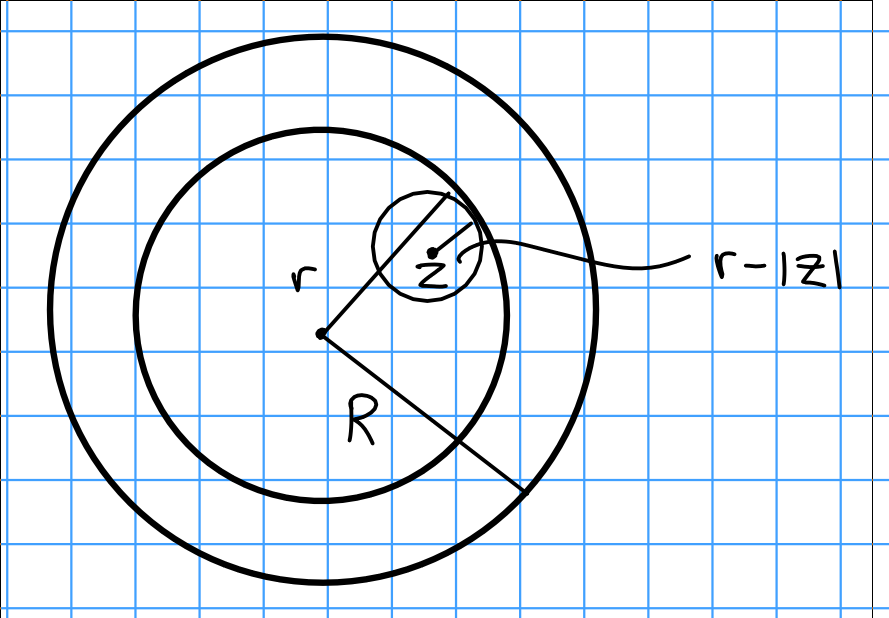
\includegraphics{figures/2020-01-17-14:14.png}
\caption{Image}
\end{figure}

We want to show \begin{align*}
\abs{S} = \abs{\frac{f(w) - f(z)}{w - z} - \sum_{n=1} a_n n z^{n-1}} \to 0 \quad \text{as } w\to z
.\end{align*}

Idea: write everything in terms of power series. Use the fact that
\(a^n - b^n = (a-b)(a^{n-1} + a^{n-2}b + \cdots)\), and so
\(\abs{(w^k-z^k)/(w-z)} \leq k r^{k-1}\).

\begin{align*}
S 
&= \sum_{n=1} a_n \qty{ \frac{w^n - z^n}{w-z} - n z^{n-1}  } \\
&= \sum a_n \qty{ w^{n-1} + w^{n-2}z + \cdots + z^{n-1} + nz^{n-1} } \\
&=  \sum a_n \qty{ (w^{n-1} - z^{n-1}) + (w^{n-2} - z^{n-2})z + \cdots + (w-z) z^{n-2} }
&= \sum a_n (w-z) \qty{ \cdots + z^{n-2} }\\
&\leq \sum_{n=2} \abs{a_n} \frac 1 2 n(n-1) r^{n-2} \abs{z-w}
.\end{align*}

\(\qed\)

Next time: trying to prove holomorphic functions are analytic.

\hypertarget{wednesday-january-22nd}{%
\section{Wednesday January 22nd}\label{wednesday-january-22nd}}

\begin{quote}
Note: multiple complex variables, see Hormander or Steven Krantz
\end{quote}

Recall from last time that if \(f(z) = \sum_{n=0}^\infty a_n z^n\) with
\(z_0 \neq 0\) has radius of convergence
\(R = (\limsup \abs{a_n}^{1/n})\inv > 0\), then \(f'\) exists and is
obtained by differentiating term-by-term. We have \(f\) analytic implies
\(f\) holomorphic (and smooth), we want to show the converse. For this,
we need integration.

\textbf{Definition:} A parameterized curve is a function \(z(t)\) which
maps a closed interval \([a, b] \subset \RR\) to \(\CC\).

\textbf{Definition:} The curve is said to be smooth iff \(z'\) exists
and is continuous on \([a,b]\), and \(z'(t) \neq 0\) for any \(t\). At
the boundary \(\theset{a, b}\), we define the derivative by taking
one-sided limits.

\textbf{Definition:} A curve is said to be piecewise smooth iff \(z(t)\)
is continuous on \([a, b]\) and there are \(a < a_1 < \cdots < a_n = b\)
with \(z\) smooth on each \([a_k, a_{k+1}]\).

\begin{quote}
Note: may fail to have tangent lines at \(a_i\).
\end{quote}

\textbf{Definition:} Two parameterizations
\(z: [a,b] \to \CC, \tilde z: [c, d] \to \CC\) are equivalent iff there
exists a \(C^1\) bijection \(s: [c, d] \to [a, b]\) where
\(s \mapsto t(s)\) such that \(s'>0\) and \(\tilde z(s) = z(s(t))\).

Note that \(s' > 0\) preserves orientation and \(s'<0\) reverses
orientation.

\textbf{Definition:}

\begin{align*}
\gamma: [a, b] \to \CC \implies \gamma^- \definedas [a,b] to \CC,~~ t \mapsto \gamma(a+b-t)
.\end{align*}

\textbf{Definition:} A curve is closed iff \(z(a) = z(b)\), and is
simple iff \(z(t) \neq z_{t_1}\) for \(t\neq t_1\).

\textbf{Definition:} For
\(C_r(z_0) \definedas \theset{z\suchthat \abs{z-z_0} = r}\), the
positive orientation is given by \(z(t) = z_0 + re^{2\pi i t}\) for
\(t\in [0, 1]\).

\textbf{Definition:} The integral of \(f\) over \(\gamma\) is defined as

\begin{align*}
\int_\gamma f ~dz = \int_a^b f(z(t)) z'(t)~dt
.\end{align*}

Note: This doesn't depend on parameterization, since if \(t = t(s)\),
then a change of variables yields

\begin{align*}
\int_\gamma f ~dz - \int_c^d f(z(t(s)))z'(t(s))t'(s) ~ds = \int_c^d f(\tilde z(s)) \tilde z'(s) ~ds
.\end{align*}

Definition: The length of \(\gamma\) is defined as
\(\abs \gamma = \int \abs{z'(t)} ~dt\).

Proposition:

\begin{enumerate}
\def\labelenumi{\arabic{enumi}.}
\item
  We can extend this definition to piecewise smooth curves by
  \begin{align*}
  \int_\gamma f~dz = \sum \int_{a_k}^{a_{k+1}} f ~dz
  \end{align*}
\item
  This integral is linear and \(\int_\gamma f = -\int_{\gamma^-} f\).
\item
  We have an inequality
\end{enumerate}

\begin{align*}
\abs{\int_\gamma f} \leq \max_{a\leq t \leq b} \abs{f(z(t))} \abs\gamma
.\end{align*}

Definition: A function \(F\) is a primitive for \(f\) on \(\Omega\) iff
\(F\) is holomorphic on \(\Omega\) and \(F'(z) = f(z)\) on \(\Omega\).

Recall that in \(\RR\), we have \(F(x) \int_a^x f(t)~dt\) as an
antiderivative with \(F'(x) = f(x)\), and \(\int f = F(b) - F(a)\).

Theorem: If \(f\) is continuous, has a primitive \(F\) in \(\Omega\),
and \(\gamma\) is a curve beginning at \(w_0\) and ending at \(w_1\),
then \(\int_\gamma f = F(w_1) - F(w_0)\).

Proof: Use definitions, write \(z(t)\) where \(z(a) = w_1, z(b) = w_2\).
Then

\begin{align*}
\int_\gamma f = \int_a^b f(z(t)) z'(t) ~ dt \\
= \int_a^b F'(z(t)) z'(t) ~dt \\
= \int_a^b F_t ~dt \\
= F(z(b)) - F(z(a)) \quad\text{by FTC}\\
= F(w_1) - F(w_2)
.\end{align*}

Note that if \(\gamma\) is piecewise smooth, the sum of the integrals
telescopes to yield the same conclusion.

\textbf{Corollary:} If \(f\) is continuous and \(\gamma\) is a closed
curve in \(\Omega\), and \(f\) has a primitive in \(\Omega\), then
\(\oint f = 0\).

\hypertarget{friday-january-24th}{%
\section{Friday January 24th}\label{friday-january-24th}}

\textbf{Corollary:} If \(\gamma\) is a closed curve on \(\Omega\) an
open set and \(f\) is continuous with a primitive in \(\Omega\) (i.e.~an
\(F\) holomorphic in \(\Omega\) with \(F'=f\)) then
\(\int_\gamma f ~dz = 0\).

\emph{Proof (easy):} \begin{align*}
\int_\gamma f ~dz = \int_\gamma F' = F'(z) z(t) ~dt  = F(z(b)) - F(z(a)) = 0
.\end{align*}

Corollary: If \(f\) is holomorphic with \(f'=0\) on \(\Omega\), then
\(f\) is constant.

\emph{Proof (easy):} Pick \(w_0 \in \Omega\); we want to fix
\(w_0 \in \Omega\) and show \(f(w) = f(w_0)\) for all \(w\in \Omega\).

Take any path \(\gamma: w_0 \to w\), then

\begin{align*}
0 = \int_\gamma f' = f(w) - f(w_0)
.\end{align*}

Example: Let \(f(z) = e^{-z^2}\), this is holomorphic. Write
\(f(z) = \sum (-1)^n z^{2n}/n!\), so
\(\int f = \sum (-1)^n z^{2n+1}/(n! (2n+1))\). Since \(f\) is entire,
\(\int f\) is entire, and \((\int f)' = f\) so this function has a
primitive. Thus \(\int_\gamma f(z) = 0\) for \emph{any} closed curve. So
take \(\gamma\) a rectangle with vertices \(\pm a , \pm a + ib\).

\begin{figure}
\centering
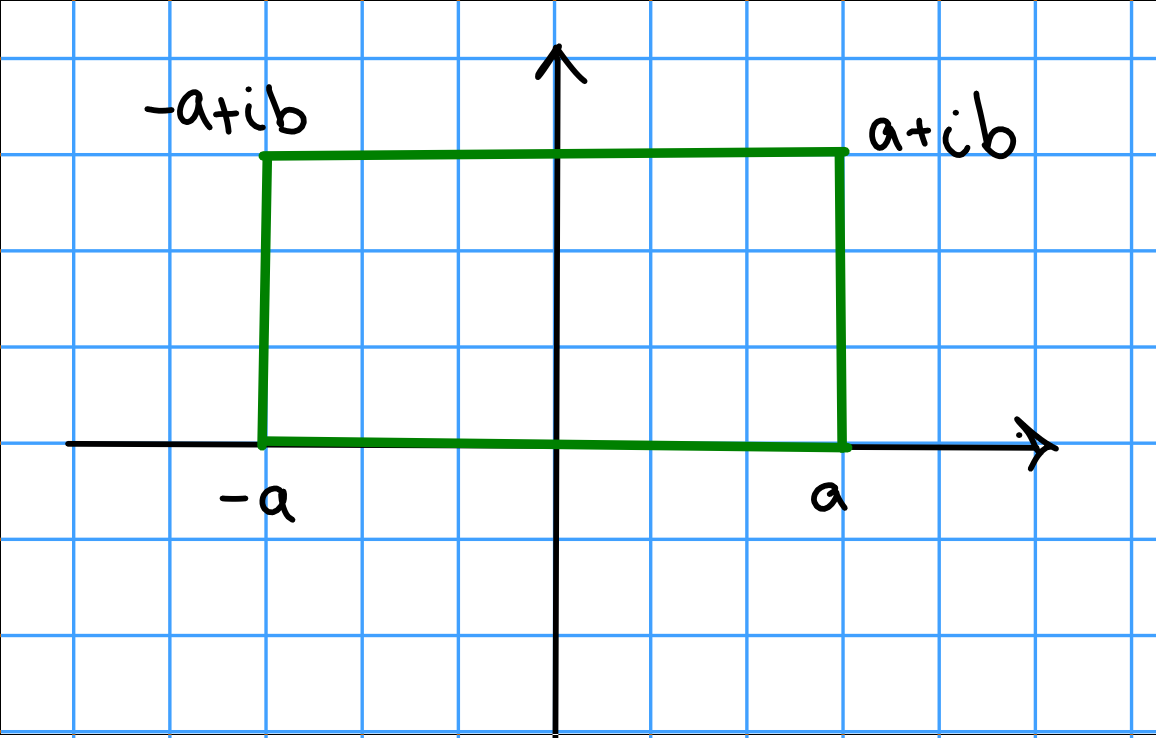
\includegraphics{figures/2020-01-24-13:36.png}
\caption{Image}
\end{figure}

So

\begin{align*}
\int_\gamma f = \int_{-a}^a e^{-x^2} ~dx + \int e^{-(a+iy)^2} i ~dy - \int_{-a}^a e^{-(x+ib)^2} ~dx - \int_0^b e^{-(a+iy)^2} i dy = 0
.\end{align*}

We can do some estimates,

\begin{align*}
e^{-(a+iy)^2} = e^{-(a^2 + 2iay - y^2)} = e^{-a^2 + y^2} e^{2iay} \leq e^{-a^2 + y^2} \leq e^{-a^2 + b^2} \\
\abs {\int_0^b e^{-(a+ib)^2} i ~dy} \leq e^{-a^2 + b^2} \cdot b \\
\int_{-a}^a e^{-(x^2 + 2ib x)-b^2} = e^{b^2} \int_{-a}^a e^{-x^2} ( \cos(2bx) - i \sin(2bx) ) \equalsbecause{odd fn} e^{b^2} \int_{-a}^a e^{-x^2} \cos(2bx) ~dx
.\end{align*}

Now take \(a\to \infty\) to obtain

\begin{align*}
\int_\RR e^{-x^2} ~dx - e^{b^2} \int_\RR e^{-x^2} \cos(2bx) ~dx
.\end{align*}

We can compute

\begin{align*}
\int_\RR e^{-x^2} = \left[ \qty{\int_\RR e^{-x^2}}^2 \right]^{1/2} = \qty{ \int_0^{2\pi} \int_0^\infty e^{r^2} r~dr~d\theta} = \sqrt{\pi}
.\end{align*}

and then conclude

\begin{align*}
\int_\RR e^{-x^2} \cos(2bx) \sqrt{\pi} e^{-b^2}
.\end{align*}

Make a change of variables \(2b = 2\pi \xi\), so \(b = \pi \xi\), then

\begin{align*}
\int_\RR e^{-x^2} \cos(2\pi \xi x) ~dx = \sqrt{\pi} e^{-\pi^2 \xi^2}
.\end{align*}

Thus \(\mcf(e^{-x^2}) = \sqrt{\pi} e^{-\pi^2 \xi^2}\), allowing
computation of the Fourier transform. Note that this can be used to
prove the Fourier inversion formula.

\textbf{Exercise:} Show that this is an approximate identity and prove
the Fourier inversion formula.

\textbf{Exercise:} Show
\(\mcf(e^{-ax^2}) = \sqrt{\pi/a} e^{-\pi^2/a \cdot \xi^2}\), and thus
taking \(a = \pi\) makes \(e^{\pi x^2}\) is an eigenfunction of \(\mcf\)
with eigenvalue \(1\).

Theorem: If \(f\) has a primitive on \(\Omega\) then \(F(z)\) is
holomorphic and \(\int_\gamma f = 0\). If \(f\) is holomorphic, then
\(\int_\gamma f = 0\).

\textbf{Theorem (Green's):} Take \(\Omega \in \RR^2\) bounded with
\(\bd \Omega\) piecewise smooth. If \(f, g\in C^1{\bar \Omega}\), then

\begin{align*}
\int_{\bd \Omega} f ~dx + g ~dy = \iint_{\Omega} \qty{g_x - f_y} ~dA
.\end{align*}

Proof: Not given here!

\textbf{Proof of Theorem}: Write \(\gamma = \bd \Gamma\), and noting
that \(f_z = f_x = \frac 1 i f_y\) implies that \(\dd{f}{\bar z}\), so

\begin{align*}
\int_\gamma f ~dz = \int_\gamma f(z) ~(dx + i dy) \\
= \int f(z) ~dx + i f(z) ~dy \\
= \iint_\Gamma \qty{if_x - f_y} ~dA \\
= i \iint_\Gamma \qty{f_x - \frac 1 i f_y} ~dA \\
= i \iint 0 ~dA = 0
.\end{align*}

Next class: We'll prove that this integral over any triangle is zero by
a limiting process.

\hypertarget{appendix}{%
\section{Appendix}\label{appendix}}

\begin{quote}
Collection of facts used on problem sets
\end{quote}

\textbf{Standard forms of conic sections:}

\begin{itemize}
\tightlist
\item
  Circle: \(x^2 + y^2 = r^2\)
\item
  Ellipse: \(\qty{\frac x a}^2 + \qty{\frac y b}^2 = 1\)
\item
  Hyperbola: \(\qty{\frac x a}^2 - \qty{\frac y b}^2 = 1\)

  \begin{itemize}
  \tightlist
  \item
    Rectangular Hyperbola: \(xy = \frac{c^2}{2}\).
  \end{itemize}
\item
  Parabola: \(-4ax + y^2 = 0\).
\end{itemize}

\begin{quote}
Mnemonic: Write \(f(x, y) = Ax^2 + Bxy + Cy^2 + \cdots\), then consider
the discriminant \(\Delta = B^2 - 4AC\):

\begin{itemize}
\tightlist
\item
  \(\Delta < 0 \iff\) ellipse

  \begin{itemize}
  \tightlist
  \item
    \(\Delta < 0\) and \(A=C, B=0 \iff\) circle
  \end{itemize}
\item
  \(\Delta = 0 \iff\) parabola
\item
  \(\Delta > 0 \iff\) hyperbola
\end{itemize}
\end{quote}

\textbf{Completing the square:}

\begin{align*}
x^2 - bx = (x - s)^2 - s^2 \quad\text{where} s = \frac{b}{2} \\
x^2 + bx = (x + s)^2 - s^2 \quad\text{where} s = \frac{b}{2}
.\end{align*}

\textbf{Useful Properties}

\begin{itemize}
\tightlist
\item
  \(\Re(z) = \frac 1 2 (z + \bar z)\) and
  \(\Im(z) = \frac{1}{2i}(z - \bar z)\).
\item
  \(z\bar z = \abs{z}^2\)
\item
  \(\cos(\theta) = \frac 1 2 \qty{e^{i\theta} + e^{-i\theta}}\)
\item
  \(\sin(\theta) = \frac{1}{2i}\qty{e^{i\theta} - e^{-i\theta}}\).
\end{itemize}

\textbf{Useful Series}

\textbackslash begin\{aligned\} \sum\emph{\{k=1\}\^{}\{n\} k
\&=\frac{n(n+1)}{2} \textbackslash{} \sum}\{k=1\}\^{}\{n\} k\^{}\{2\}
\&=\frac{n(n+1)(2 n+1)}{6} \textbackslash{} \sum\_\{k=1\}\^{}\{n\}
k\^{}\{3\} \&=\frac{n^{2}(n+1)^{2}}{4} \textbackslash end\{aligned\}

\textbf{Cauchy-Riemann Equations}

\begin{align*}
u_x = v_y \quad\text{and}\quad u_y = -v_x \\
\frac{\partial u}{\partial r}=\frac{1}{r} \frac{\partial v}{\partial \theta} \quad \text { and } \quad \frac{\partial v}{\partial r}=-\frac{1}{r} \frac{\partial u}{\partial \theta} \\
.\end{align*}

\hypertarget{useful-techniques}{%
\subsection{Useful Techniques}\label{useful-techniques}}

\textbf{Showing a function is constant:} Write \(f = u + iv\) and use
Cauchy-Riemann to show \(u_x, u_y = 0\), etc.

\textbf{Deriving Polar Cauchy-Riemann:} See
\href{https://users.math.msu.edu/users/shapiro/Teaching/classes/425/crpolar.pdf}{walkthrough
here}. Take derivative along two paths, along a ray with constant angle
\(\theta_0\) and along a circular arc of constant radius \(r_0\). Then
equate real and imaginary parts. See problem set 1.

Computing Arguments: \(\Arg(z/w) = \Arg(z) - \Arg(w)\).

The sum of the interior angles of an \(n\dash\)gon is \((n-2)\pi\),
where each angle is \(\frac{n-2}{n}\pi\).

%\listoftodos

\bibliography{/home/zack/Notes/library.bib}

\end{document}
